% =============================================================================
%  figures/example-figure/example-figure.tex
%  STANDALONE TikZ source of the example figure.
%  Compile this file by itself to produce example-figure.pdf (same name):
%      cd figures/example-figure
%      xelatex example-figure.tex
%  The compiled PDF is included directly in the paper with
%  
\includegraphics{example-figure/example-figure.pdf}.
%
%  Recommended figure workflow: one folder per figure, containing the
%  standalone TikZ source and its compiled PDF, both with the same name.
%  图片工作流：每张图一个子目录，TikZ 源文件与编译产物同名同处。
%
%  The drawing below is a GENERIC example (a stylized two-series line chart)
%  and is unrelated to any research topic -- replace it with your own figure.
% =============================================================================

\documentclass[border=8pt]{standalone}

\usepackage{tikz}
\usetikzlibrary{calc,positioning}
\definecolor{winered}{rgb}{0.5,0,0}   % match main.tex link color

\begin{document}

% GENERIC PLACEHOLDER FIGURE: two dummy series plotted against time.
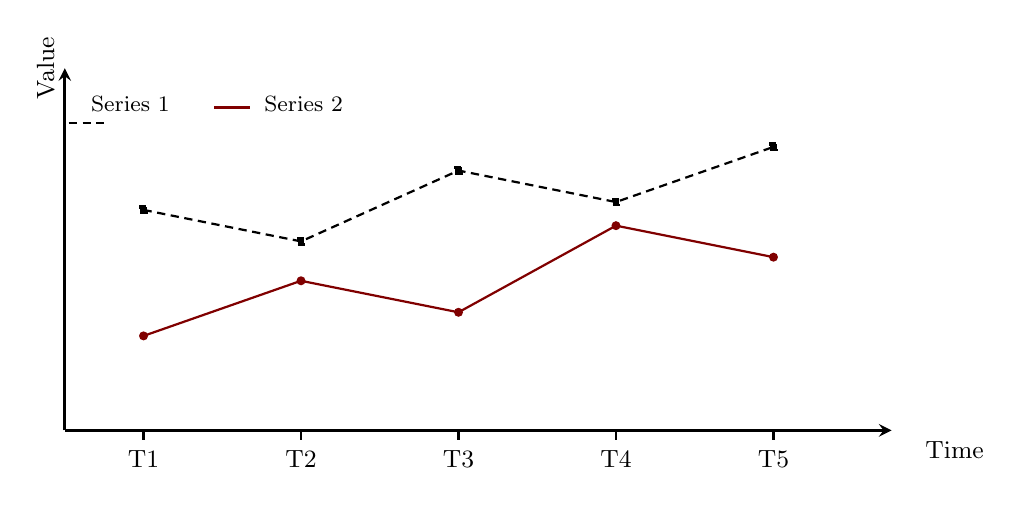
\begin{tikzpicture}[
    font=\small,
    >=stealth,
    line width=1pt
  ]
  % axes
  \draw[->] (0,0) -- (10.5,0) node[below, xshift=0.8cm] {Time};
  \draw[->] (0,0) -- (0,4.6) node[above, rotate=90, anchor=south] {Value};

  % tick labels (generic)
  \foreach \x/\lab in {1/T1, 3/T2, 5/T3, 7/T4, 9/T5}
    \draw (\x,0) -- (\x,-0.12) node[below] {\lab};

  % series 1
  \draw[winered, thick]
    plot[mark=*, mark size=1.2pt] coordinates
      {(1,1.2) (3,1.9) (5,1.5) (7,2.6) (9,2.2)};

  % series 2
  \draw[black, thick, densely dashed]
    plot[mark=square*, mark size=1.2pt] coordinates
      {(1,2.8) (3,2.4) (5,3.3) (7,2.9) (9,3.6)};

  % legend (generic)
  \node[anchor=west, font=\footnotesize] at (0.2,4.15) {Series 1};
  \node[anchor=west, font=\footnotesize] at (2.4,4.15) {Series 2};
  \draw[winered, thick] (1.9,4.1) -- (2.35,4.1);
  \draw[black, thick, densely dashed] (0.05,3.9) -- (0.5,3.9);
\end{tikzpicture}

\end{document}
